% !TEX encoding = UTF-8
% !TEX TS-program = pdflatex
% !TEX root = ../Relazione.tex
% !TEX spellcheck = it-IT

%%%%%%%%%%%%%%%%%%%%%%%
\section{Network breakdown}
\label{sec:attaack}
%%%%%%%%%%%%%%%%%%%%%%%
%(formerly "Analisi percolativa" ma questo è un titolo noioso, meglio una roba più deep impact ogliea) 

Una volta osservate le distribuzioni del grado nelle reti delle quattro compagnie e nella rete complessiva formata da tutte le antenne comprese nell'area metropolitana di Roma, procediamo con lo studio percolativo. In riferimento al lavoro fatto da \textcite{Barbalbert2000}, la scelta è stata di simulare due differenti scenari in cui i nodi della rete vengono disabilitati. Nel primo scenario si è ipotizzato un attacco intenzionale che cominciasse dai nodi con maggior grado, nel secondo una rimozione random. 

Lo scopo è studiare l'andamento, in funzione della percentuale di nodi rimossi, del diametro $D$ della rete e della dimensione del cluster più grande (ipotizzando, o meglio verificando, che esso sia il Giant Cluster della rete) rapportata al numero totale di nodi sopravvissuti. A seconda di come la rete si comporterà, sarà possibile dedurne la robustezza nei due scenari, in modo tale da poter confrontare meglio tale comportamento con quello di una rete scale-free o random, di pari grado medio $\langle k \rangle$.

In tutti e cinque i campioni di rete che abbiamo analizzato sono stati conteggiati gli andamenti di alcune grandezze topologiche e statistiche di interesse: dimensione del giant cluster, $D$ e $\langle l \rangle$, coefficiente di clustering globale $C$, $\langle k \rangle$ e $\langle k^2 \rangle/\langle k \rangle$. I grafici ottenuti sono stati messi a confronto a quelli ottenuti con le reti generate secondo i modelli.

% <!-- TODO DA DECIDERE SE TAGLIARE O SINTETIZZARE  -->
La rete reale ha ovviamente delle contromisure per evitare la caduta delle comunicazioni. Le antenne trasmettono segnali tra loro su due bande di frequenza: una \emph{user-side}, dedicata alle normali trasmissioni tra utenti del servizio, e una dedicata a un complesso sistema di feedback gestito da degli \emph{hub} (grosse antenne con raggio sui 20 km). Questa struttura gerarchica permette, nel caso di caduta di una antenna o di un improvviso eccessivo carico in una zona circoscritta, che gli hub gestiscano potenza e capacità delle antenne circostanti mentre vengono inviati tecnici per un intervento sul luogo.

Questo sistema ha un certo tempo di reazione. L'analisi da noi svolta pertanto suppone che la caduta della rete avvenga in un tempo inferiore, in una sorta di approssimazione adiabatica. Inoltre, la sola caduta degli hub sarebbe già sufficiente a compromettere seriamente l'integrità della rete (le antenne avrebbero difficoltà a coordinare le comunicazioni tra loro), ma nella nostra ipotesi di mesh-network distribuita ci interessano soltanto le comunicazioni nelle frequenze user-side. Usando questo modello semplificato siamo riusciti a ottenere alcune informazioni su una ipotetica rete wireless di questa natura.

\subsection{Il punto di partenza}
Le reti da cui è partito lo studio percolativo sono le 5 definite e costruite nel precedente paragrafo. Le grandezze iniziali erano


\begin{table}[t]
\caption{Dati iniziali delle reti studiate.}
	\begin{tabular}{cccccccccc}
	\toprule
	Rete		&N		&$GC\%$	&$D$	&$\langle l\rangle$	&$C$		&$\langle k\rangle$	&$C/\langle k\rangle$	&$\langle k^2\rangle/\langle k\rangle$	&$f\%$\\
	\midrule  
	Tim		&1756	&1		&2	&1.96			&0.89	&64.3			&0.014				&359							&99.7\\
	Vodafone	&1771	&1		&2	&1.97			&0.87	&52.9			&0.016				&243							&99.6\\
	Wind		&2365	&1		&2	&1.96			&0.89	&97.3			&0.009				&478							&99.8\\
	Tre		&1395	&1		&2	&1.97			&0.88	&41.4			&0.021				&239							&99.6\\
	Roma		&7287	&1		&2	&1.97			&0.89	&239.1			&0.004				&1353							&99.9\\
	\bottomrule
	\end{tabular}
\label{tab:datiInitial}
\end{table}

\subsubsection{Random failure}
La prima cosa da notare è che le reti delle singole compagnie hanno un rapporto coefficiente di clustering-grado medio in linea con molte altre reti reali \parencite{Barbalbert2002}, mentre stranamente la rete costruita con tutte le antenne non vede aumentare particolarmente il suo clustering. Inoltre ci si aspetta che le reti siano tutte particolarmente resistenti sotto random failure, comportamento che sembra più simile a quello di una rete scale free. Tuttavia una rete random con un grado medio alto ha comunque un $f$ molto alto. Per esempio, una rete random avente $N = N_{Tim}$ e $\langle k \rangle = \langle k \rangle_{Tim}$, avrebbe una $f$ critica di poco inferiore: $\sim 98\%$. Infatti, essendo per una rete random $\langle k \rangle = Np$, perché sia uguale a $\langle k \rangle_{Tim}$ con $\sim 1800$ nodi, deve essere $p \sim 3.7\%$, 
$$\Rightarrow \sigma^2 = Np(1-p) = \langle k^2 \rangle - \langle k \rangle^2 \sim 62$$
$$\Rightarrow \frac{\langle k^2 \rangle }{\langle k \rangle} = \frac{Np(1-p)-(Np)^2}{Np} \sim 1+Np = 1+ \langle k \rangle \sim 65$$
$$\Rightarrow f \sim 1 - \frac{1}{65} \sim 98\%$$

Con una rete random costruita con i parametri della rete totale si ottiene $f = 99.5$. Valori quindi che si distinguono poco dalla soglia per una rete power-law finita, anche nel caso in cui l'esponente sia di poco maggiore di 3: $f \sim 1 - \frac{1}{\frac{\alpha - 2}{\alpha-3}k_{max}} > 90\%$ già per un grado massimo di $\sim10$.


\subsubsection{Attacco intenzionale}
Nello scenario di attacco intenzionale ci si aspetta una veloce frammentazione della rete. I cluster diverranno rapidamente più piccoli fino a frammentarsi del tutto entro pochi punti percentuali di nodi rimossi. Nel caso di una rete fortemente connessa come quella in esame ci si aspetta una resistenza maggiore, ma comunque una soglia percolativa bassa (approssimativamente entro il $50\%$). Se la rete è di tipo scale-free dovrebbe essere più fragile ad attacchi di questo tipo: mentre in una rete random i nodi più connessi sono solo una coda della distribuzione del grado, una rete a power-law ha in proporzione molti più nodi molto connessi.

Dal punto di vista del diametro della rete, levando i nodi più connessi ci si aspetta che esso aumenti, fino a quando la rete diventa tanto frammentata da essere costituita da clusters con pochissimi nodi. Oltrepassata la soglia di frammentazione quindi il diametro dei clusters più grandi decrescerà rapidamente a zero.

\subsection{Risultati}
\begin{figure}[p!]
	\centering
	\subfloat[$GC$]
	{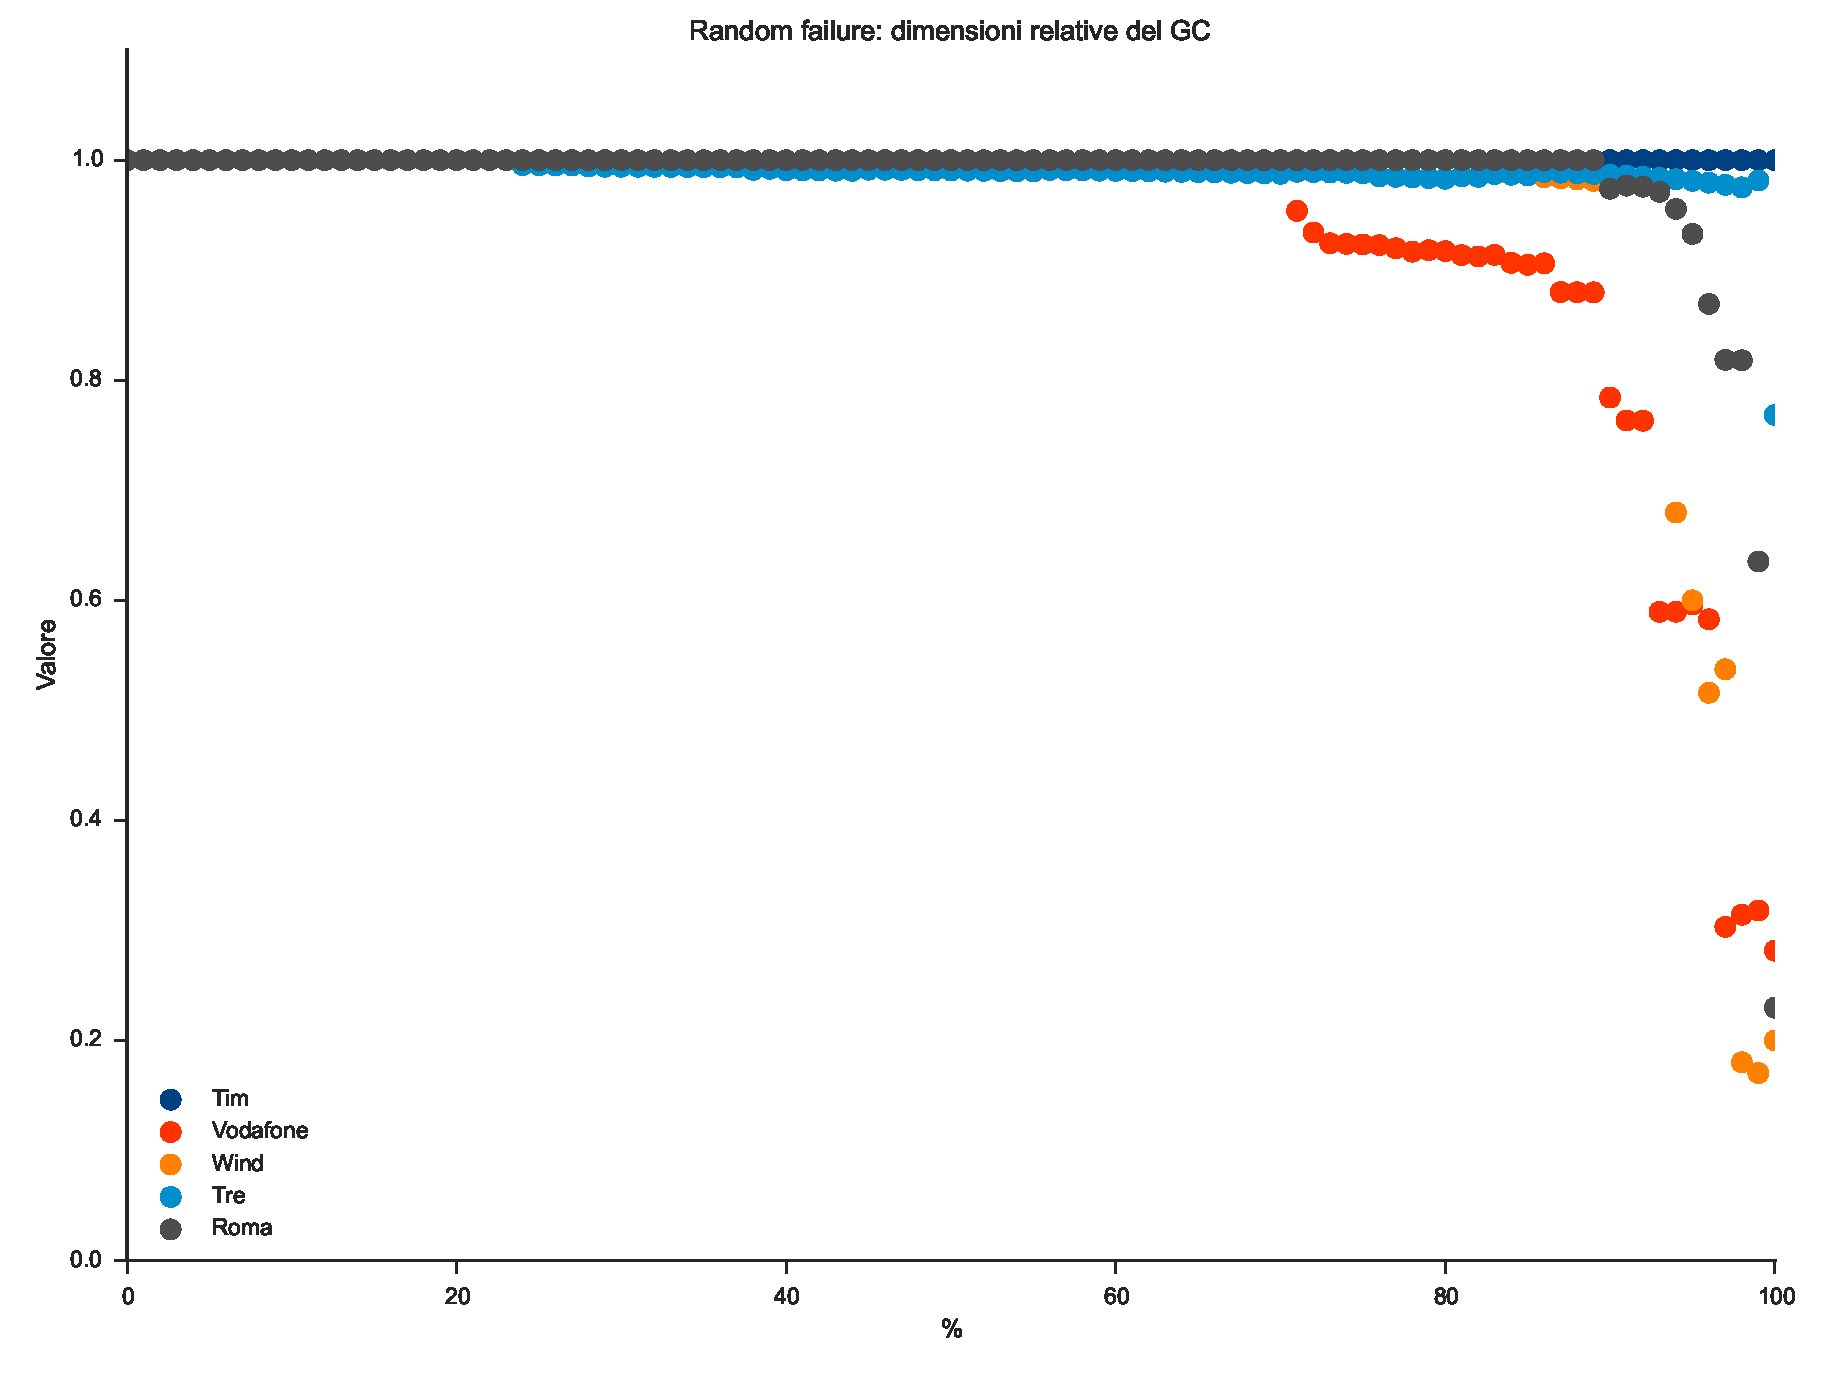
\includegraphics[width=0.46\textwidth]{./Immagini/Attack/gToolFailureGC_Final}}
	$\;$
	\subfloat[$C$]
	{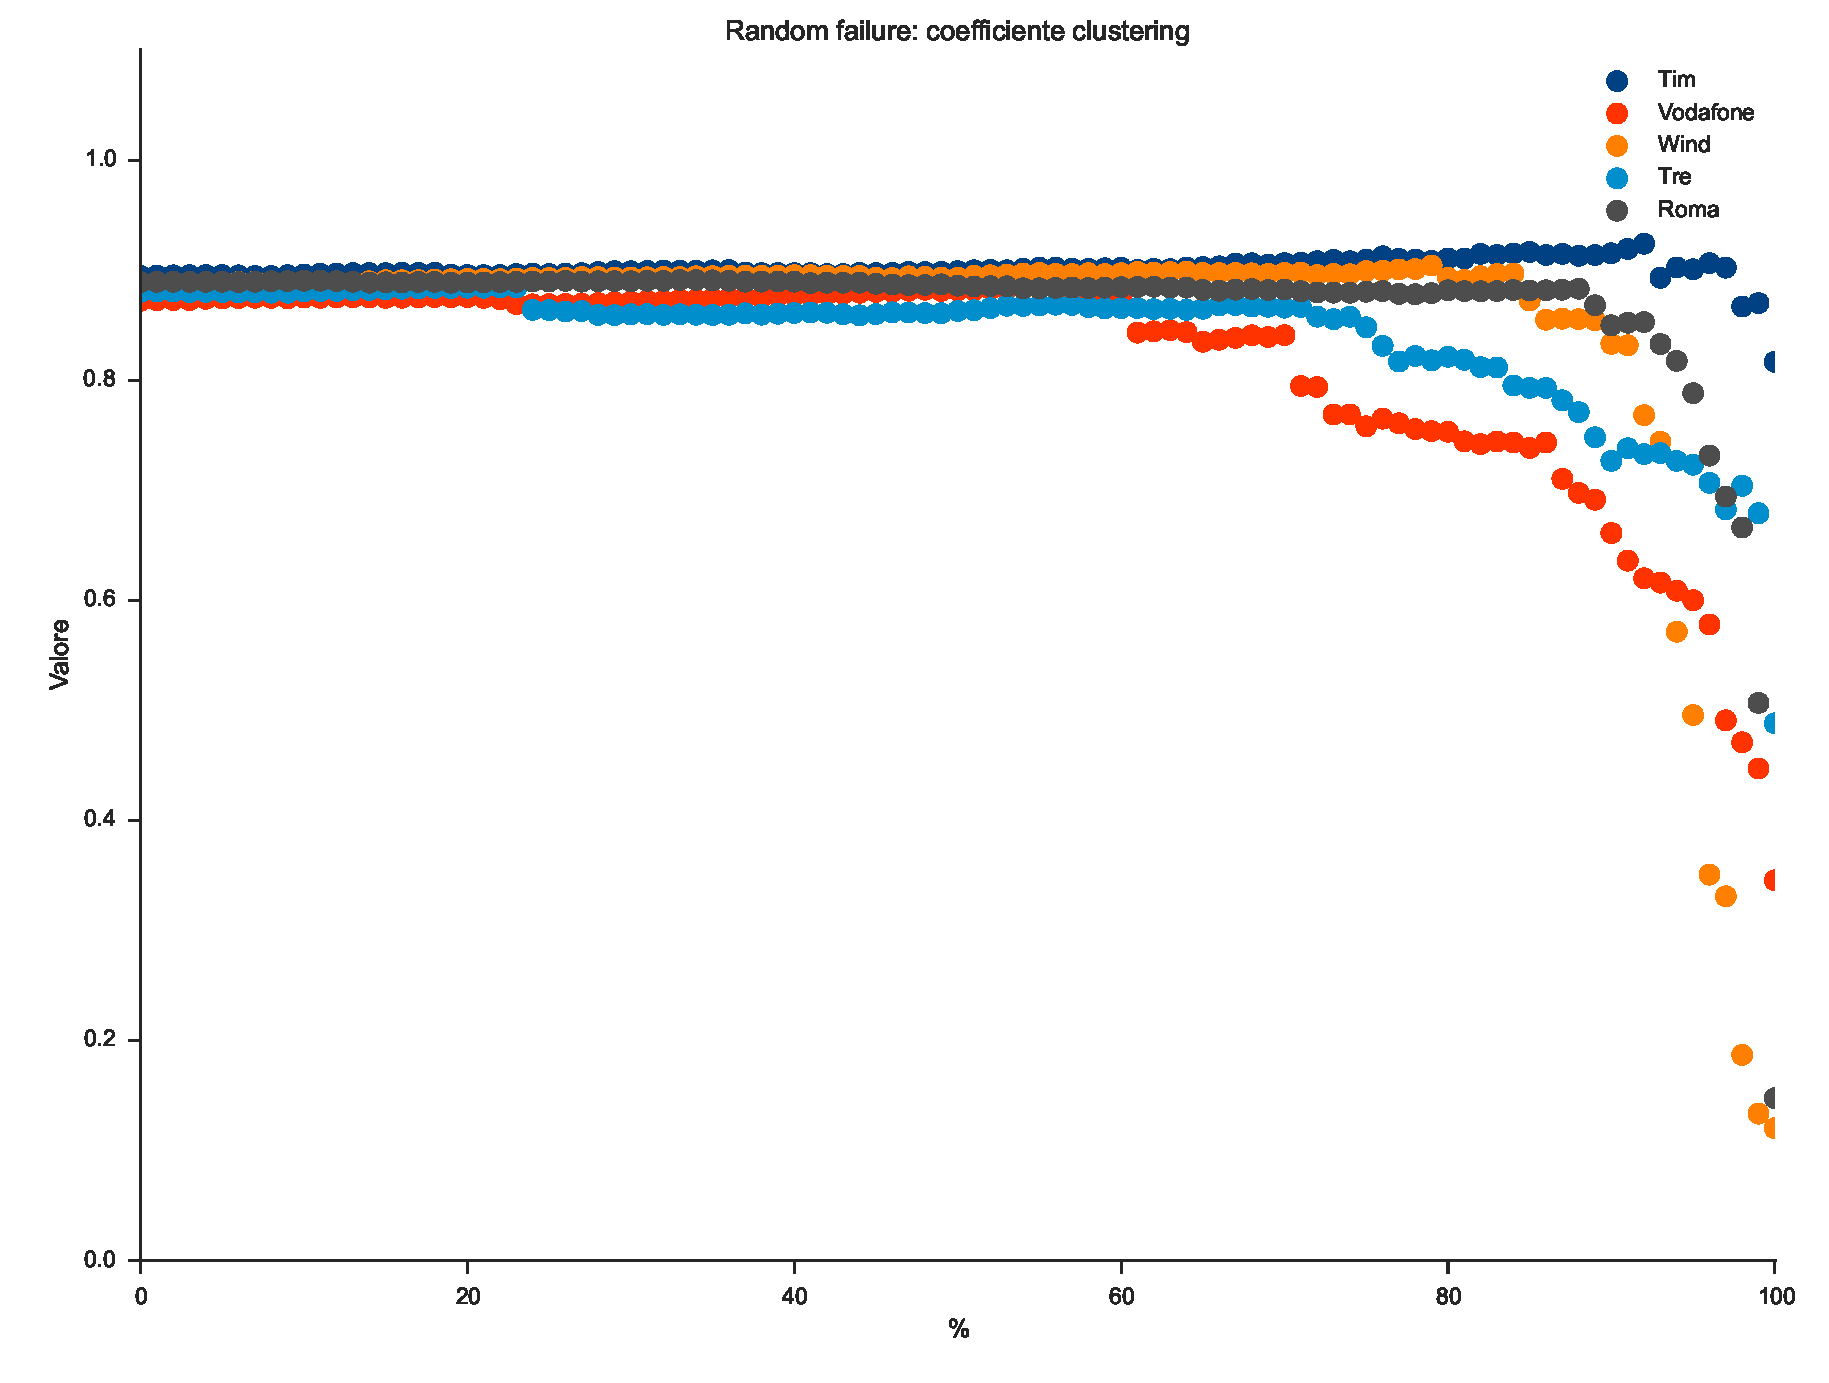
\includegraphics[width=0.46\textwidth]{./Immagini/Attack/gToolFailureC_Final}}
	\\
	\subfloat[$\langle l \rangle$]
	{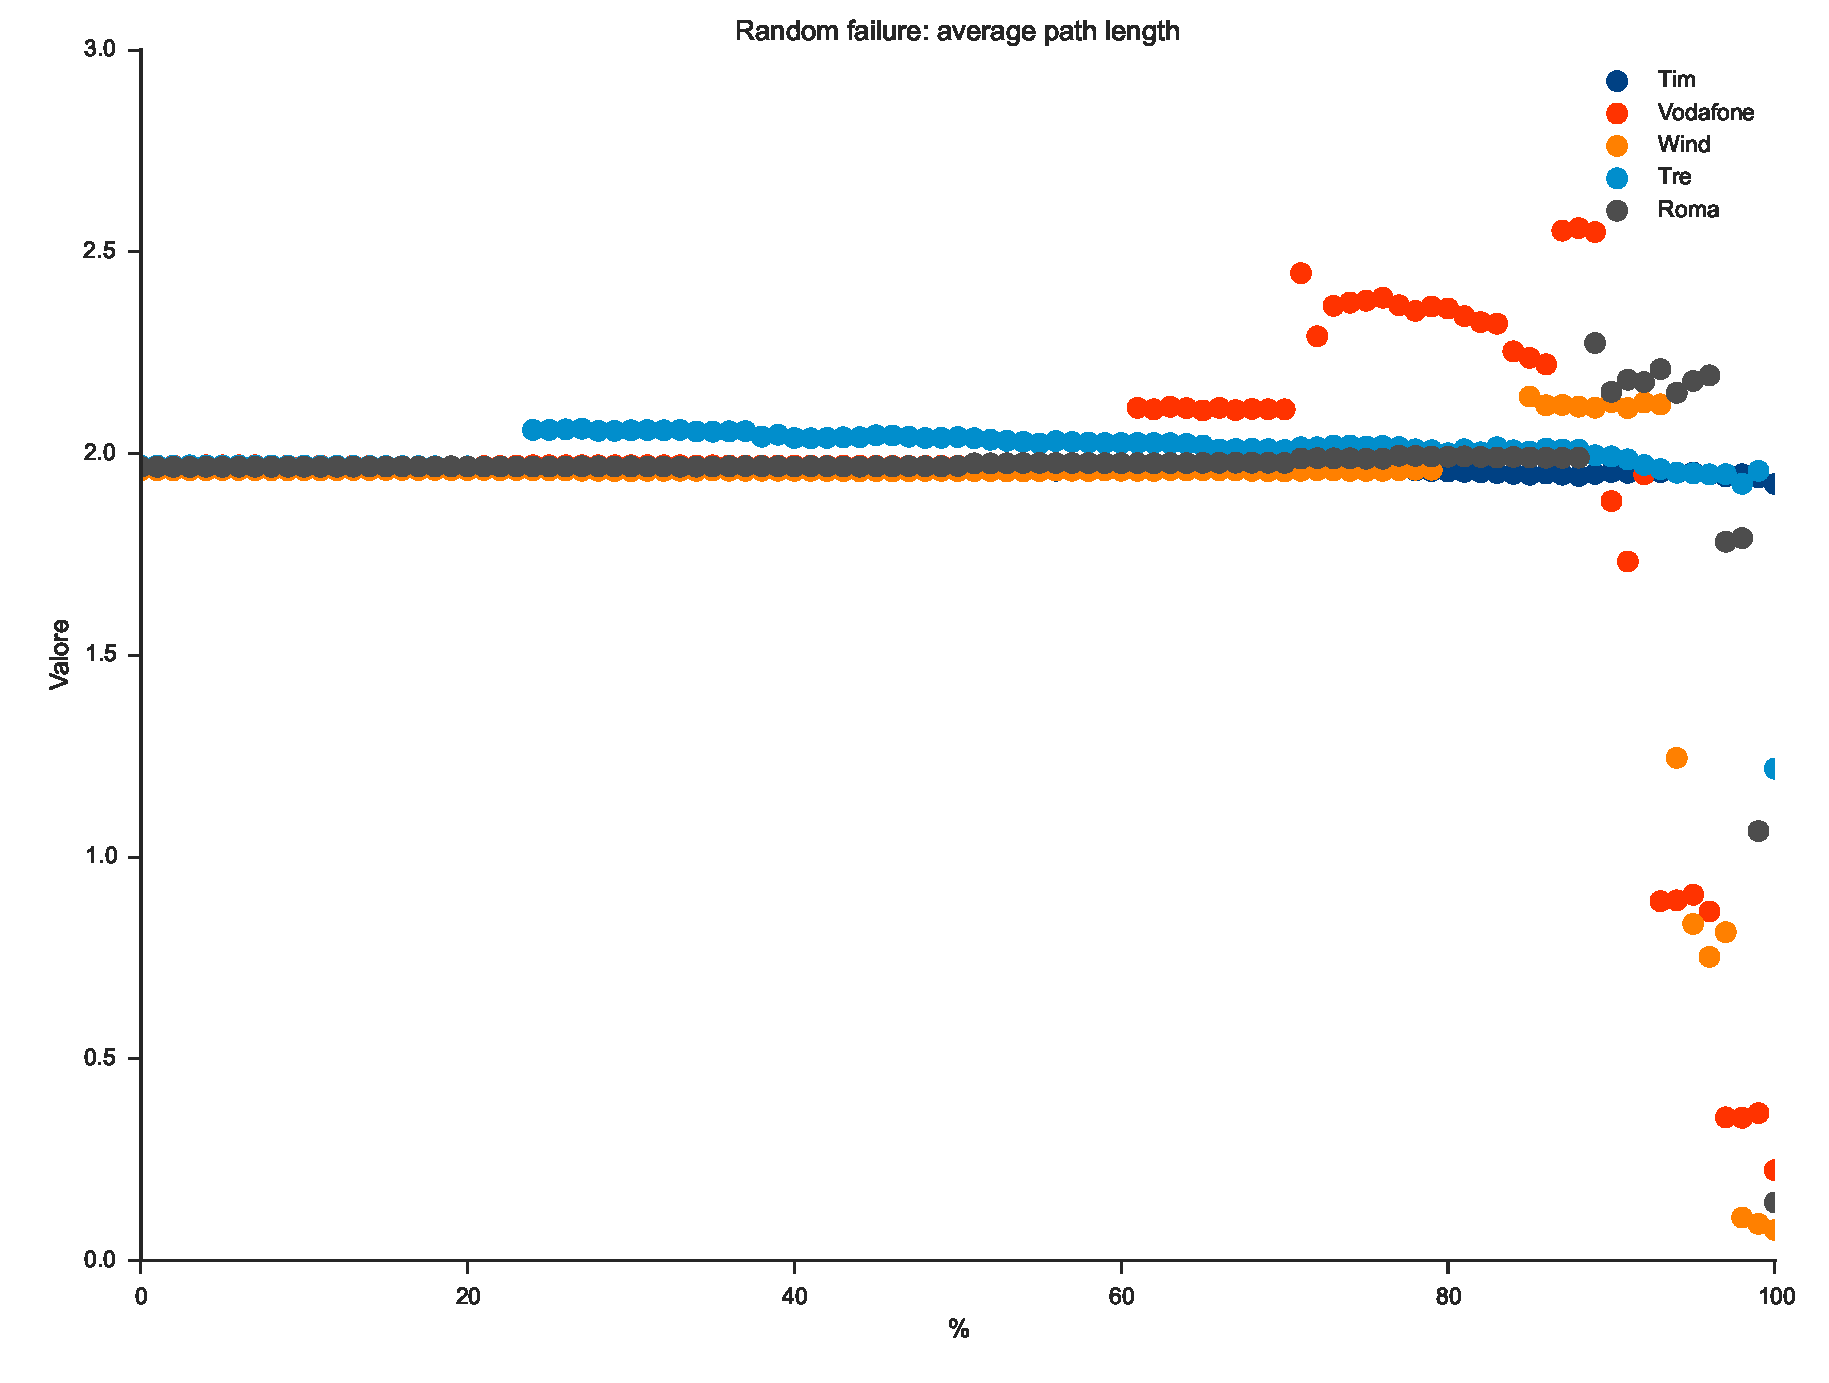
\includegraphics[width=0.46\textwidth]{./Immagini/Attack/gToolFailurel_Final}}
	$\;$
	\subfloat[$D$]
	{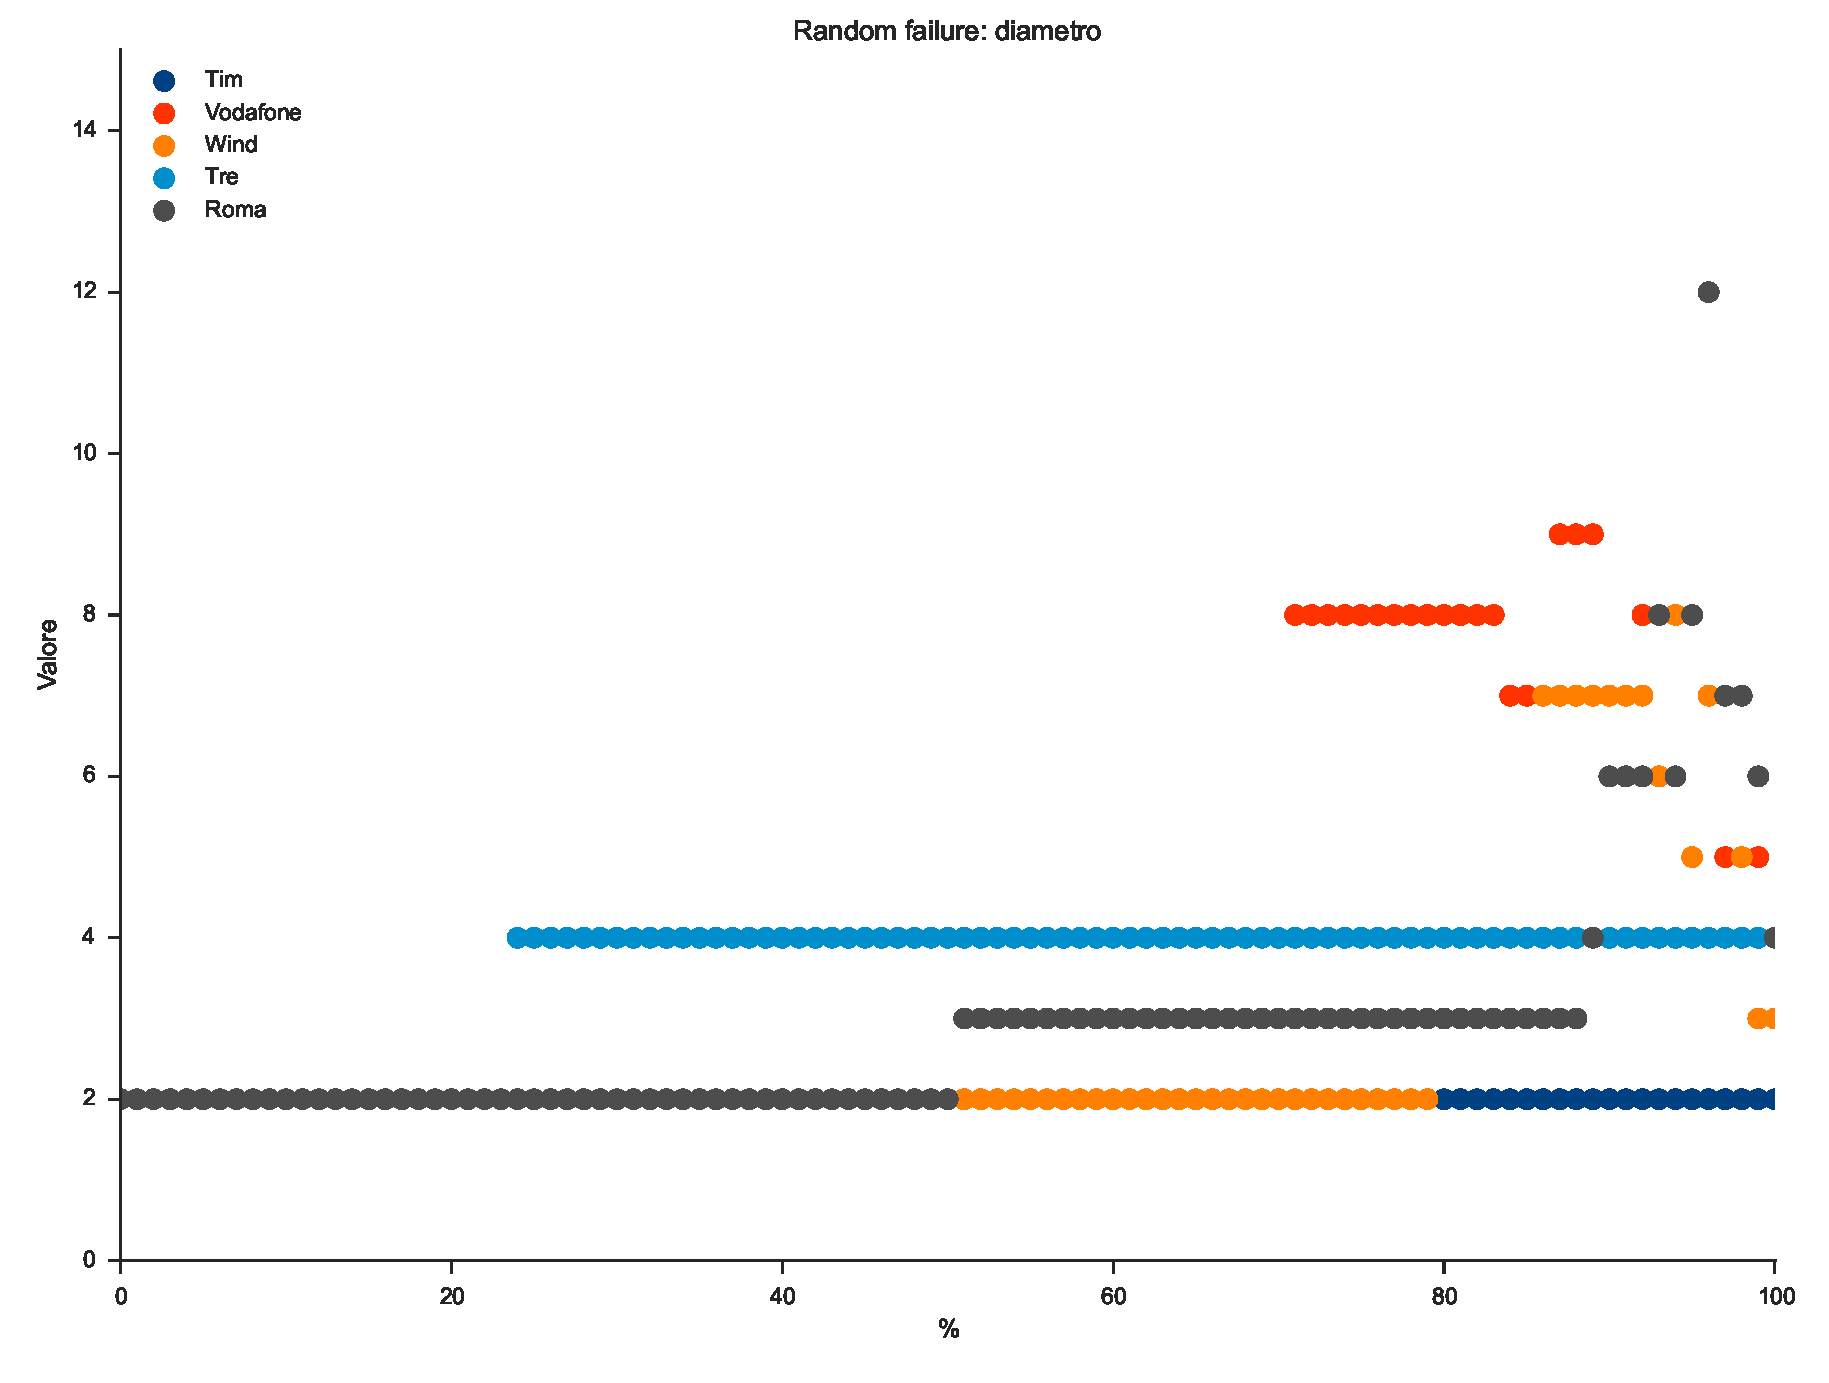
\includegraphics[width=0.46\textwidth]{./Immagini/Attack/gToolFailureD_Final}}
	\\
	\subfloat[$\langle k \rangle$]
	{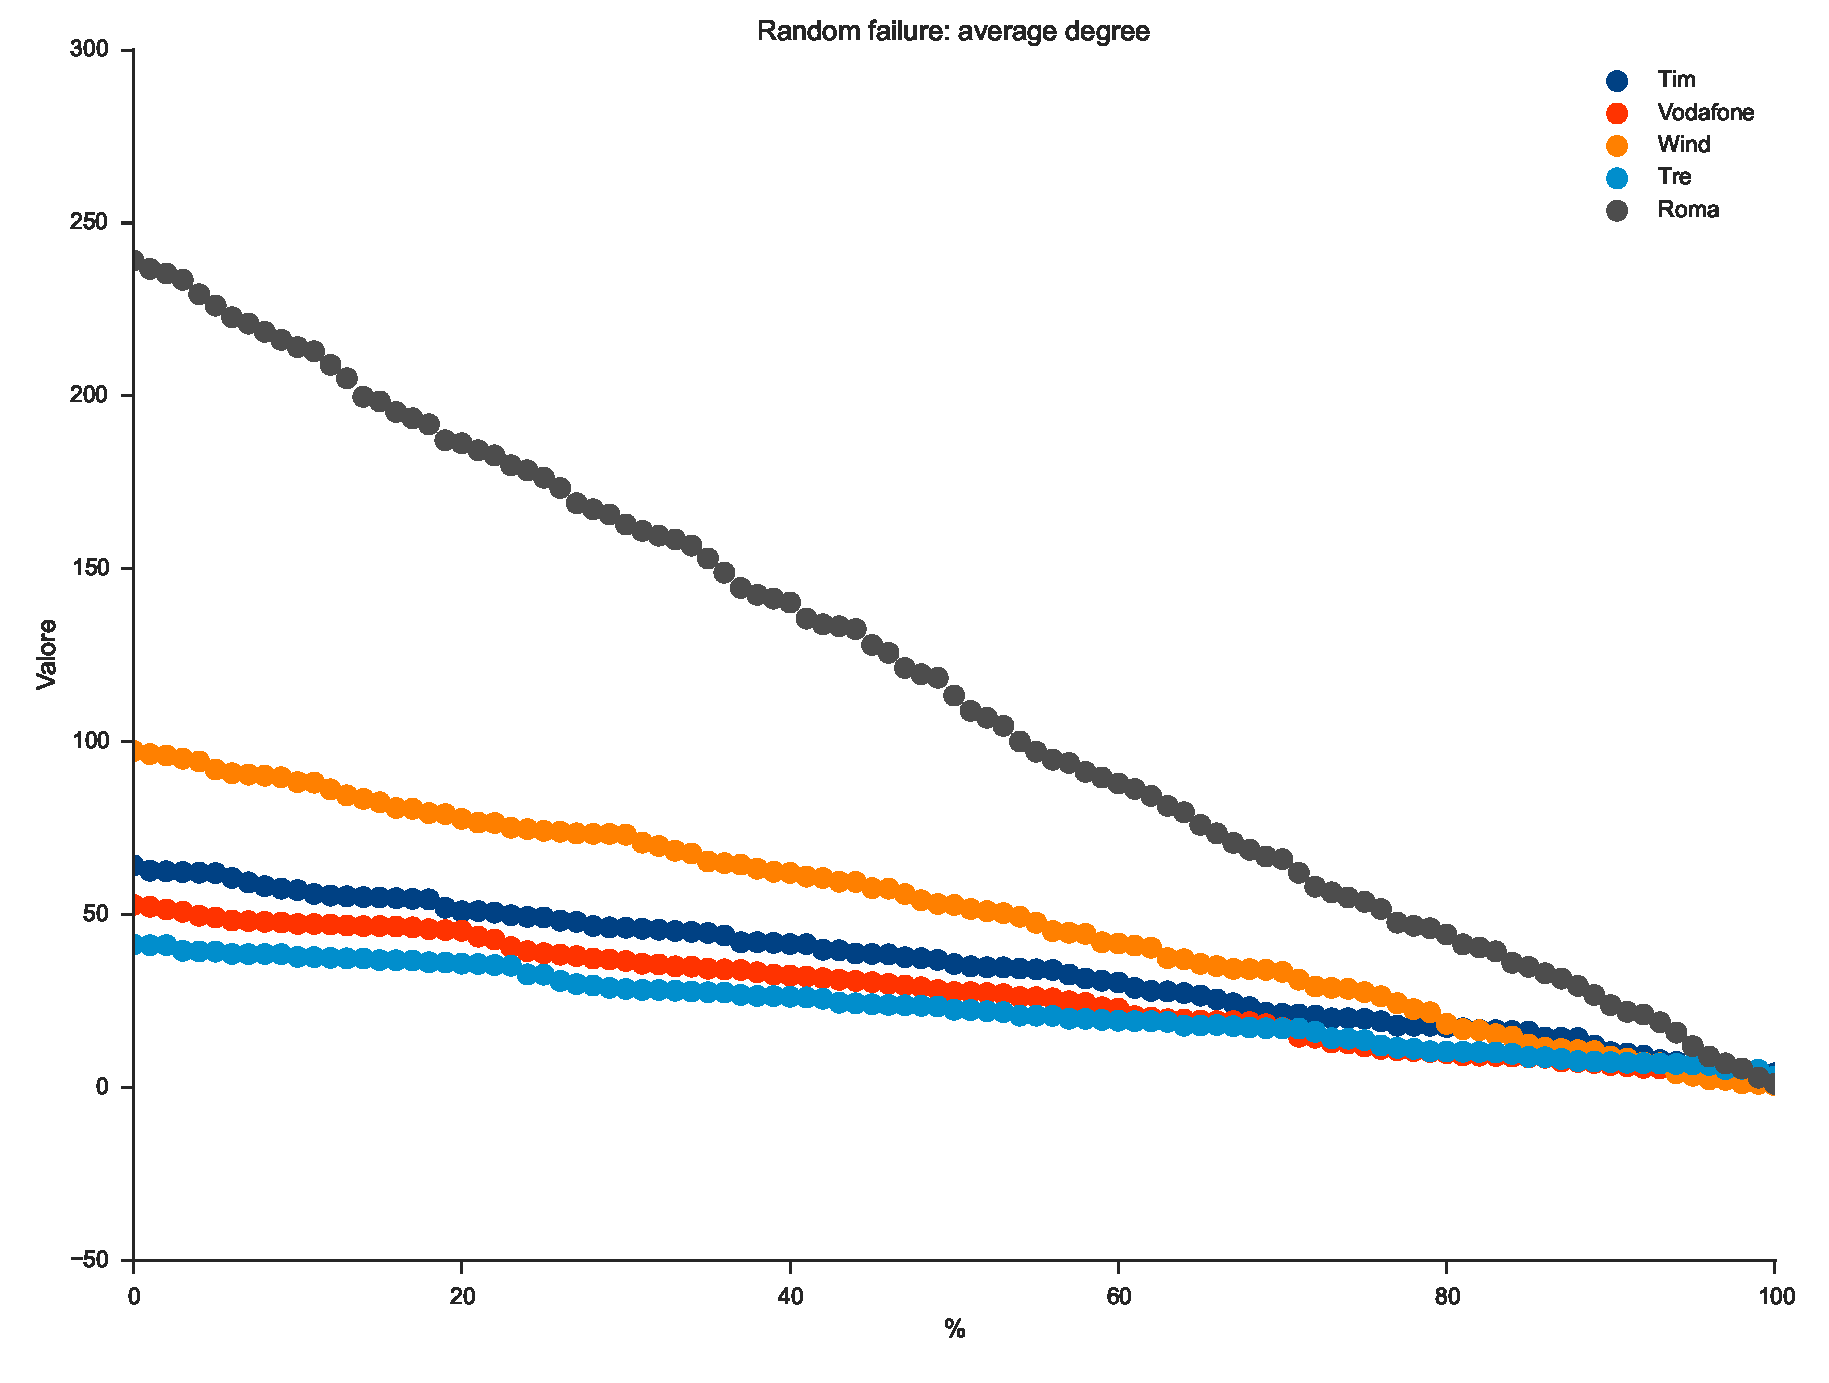
\includegraphics[width=0.46\textwidth]{./Immagini/Attack/gToolFailurek_Final}}
	$\;$
	\subfloat[$\langle k^2 \rangle/\langle k \rangle$]
	{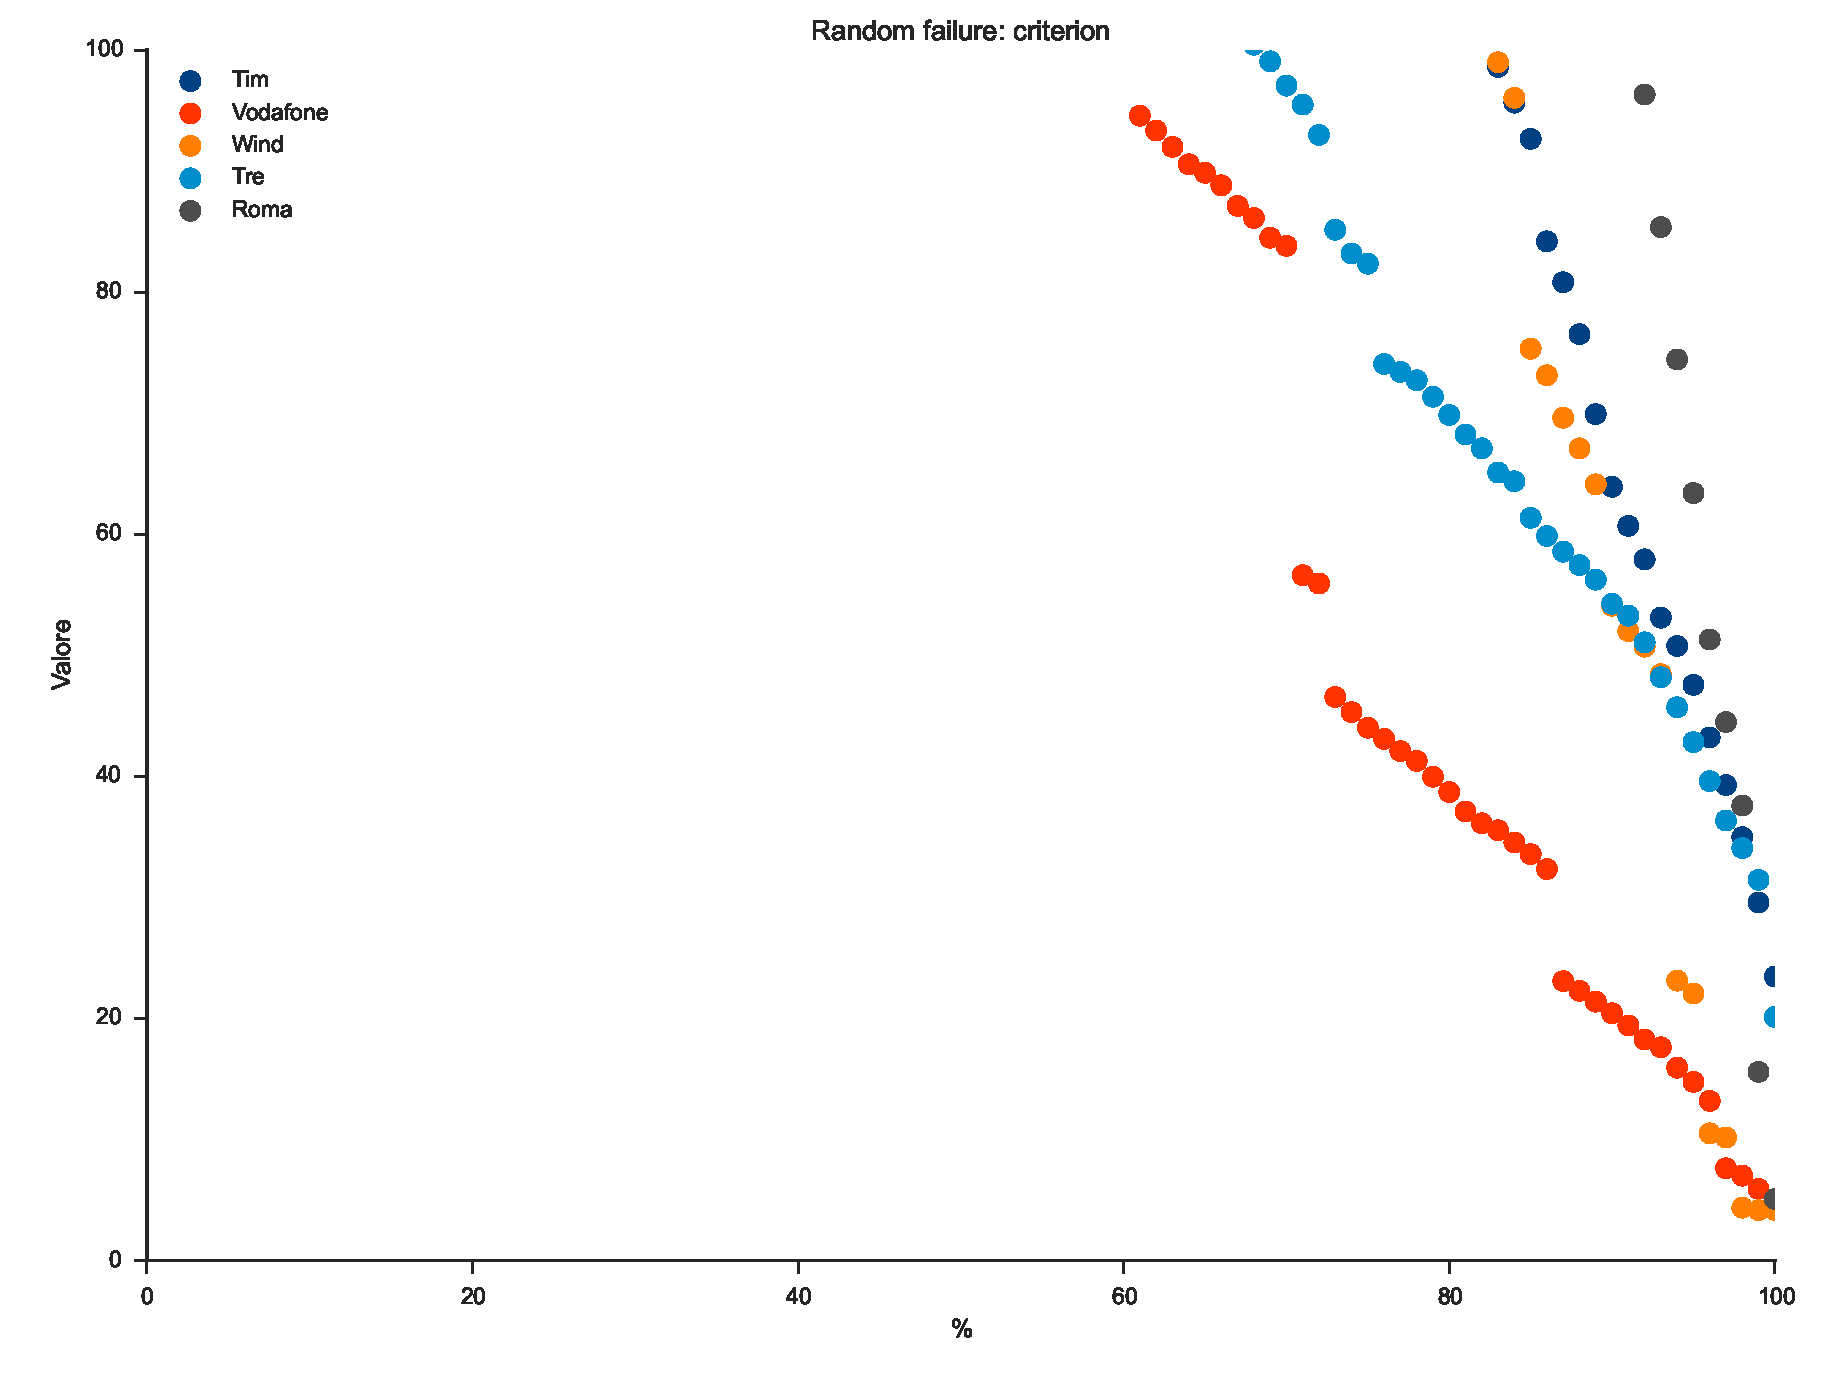
\includegraphics[width=0.46\textwidth]{./Immagini/Attack/gToolFailurec_Final}}
	\caption[Risultati random.]{Risultati per rimozione random}
	\label{fig:fail}
\end{figure}

\begin{figure}[p!]
	\centering
	\subfloat[$GC$]
	{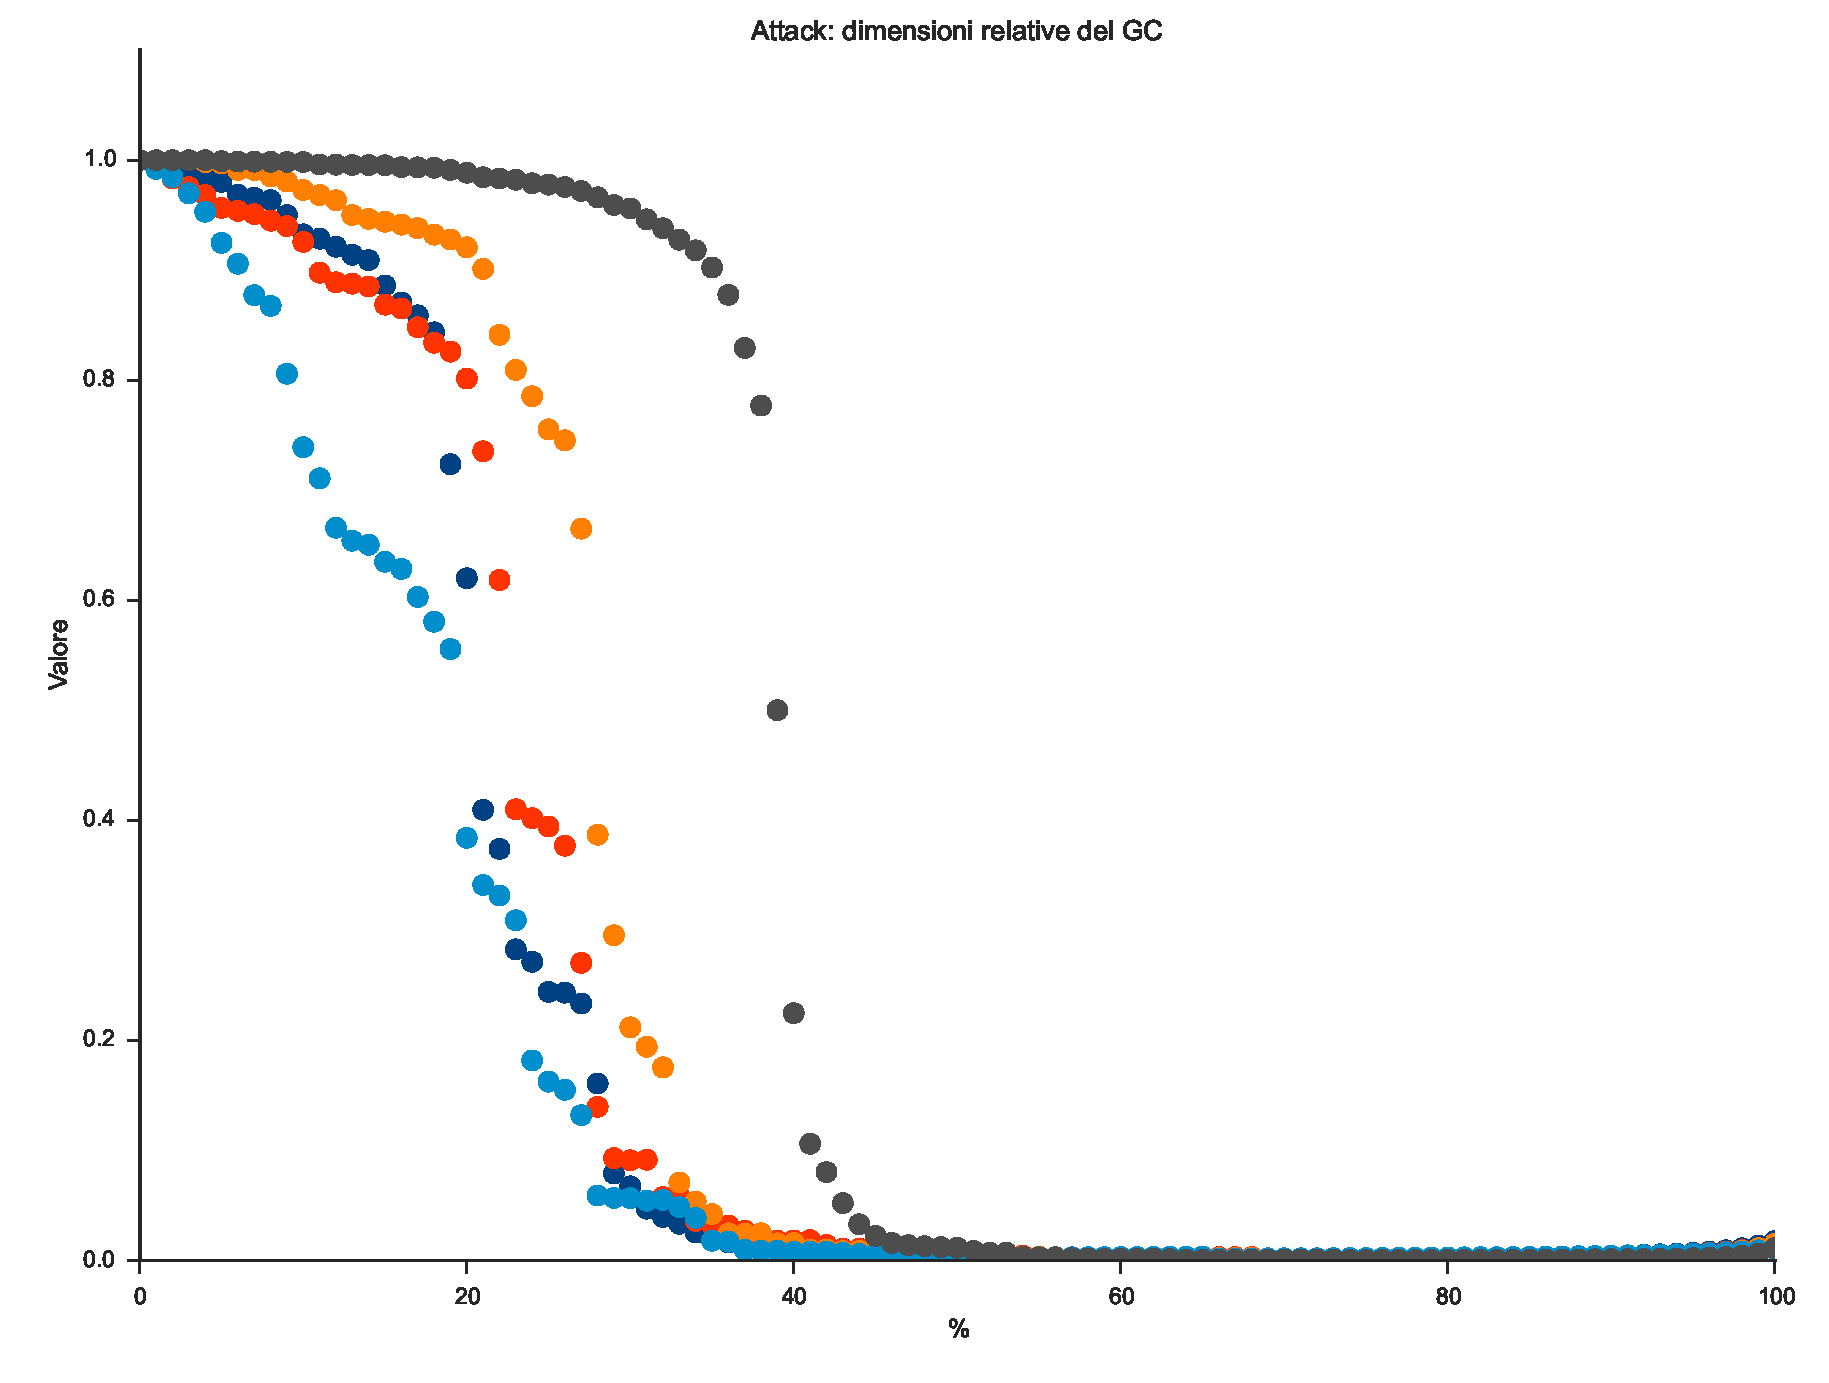
\includegraphics[width=0.46\textwidth]{./Immagini/Attack/gToolAttackGC_Final}}
	$\;$
	\subfloat[$C$]
	{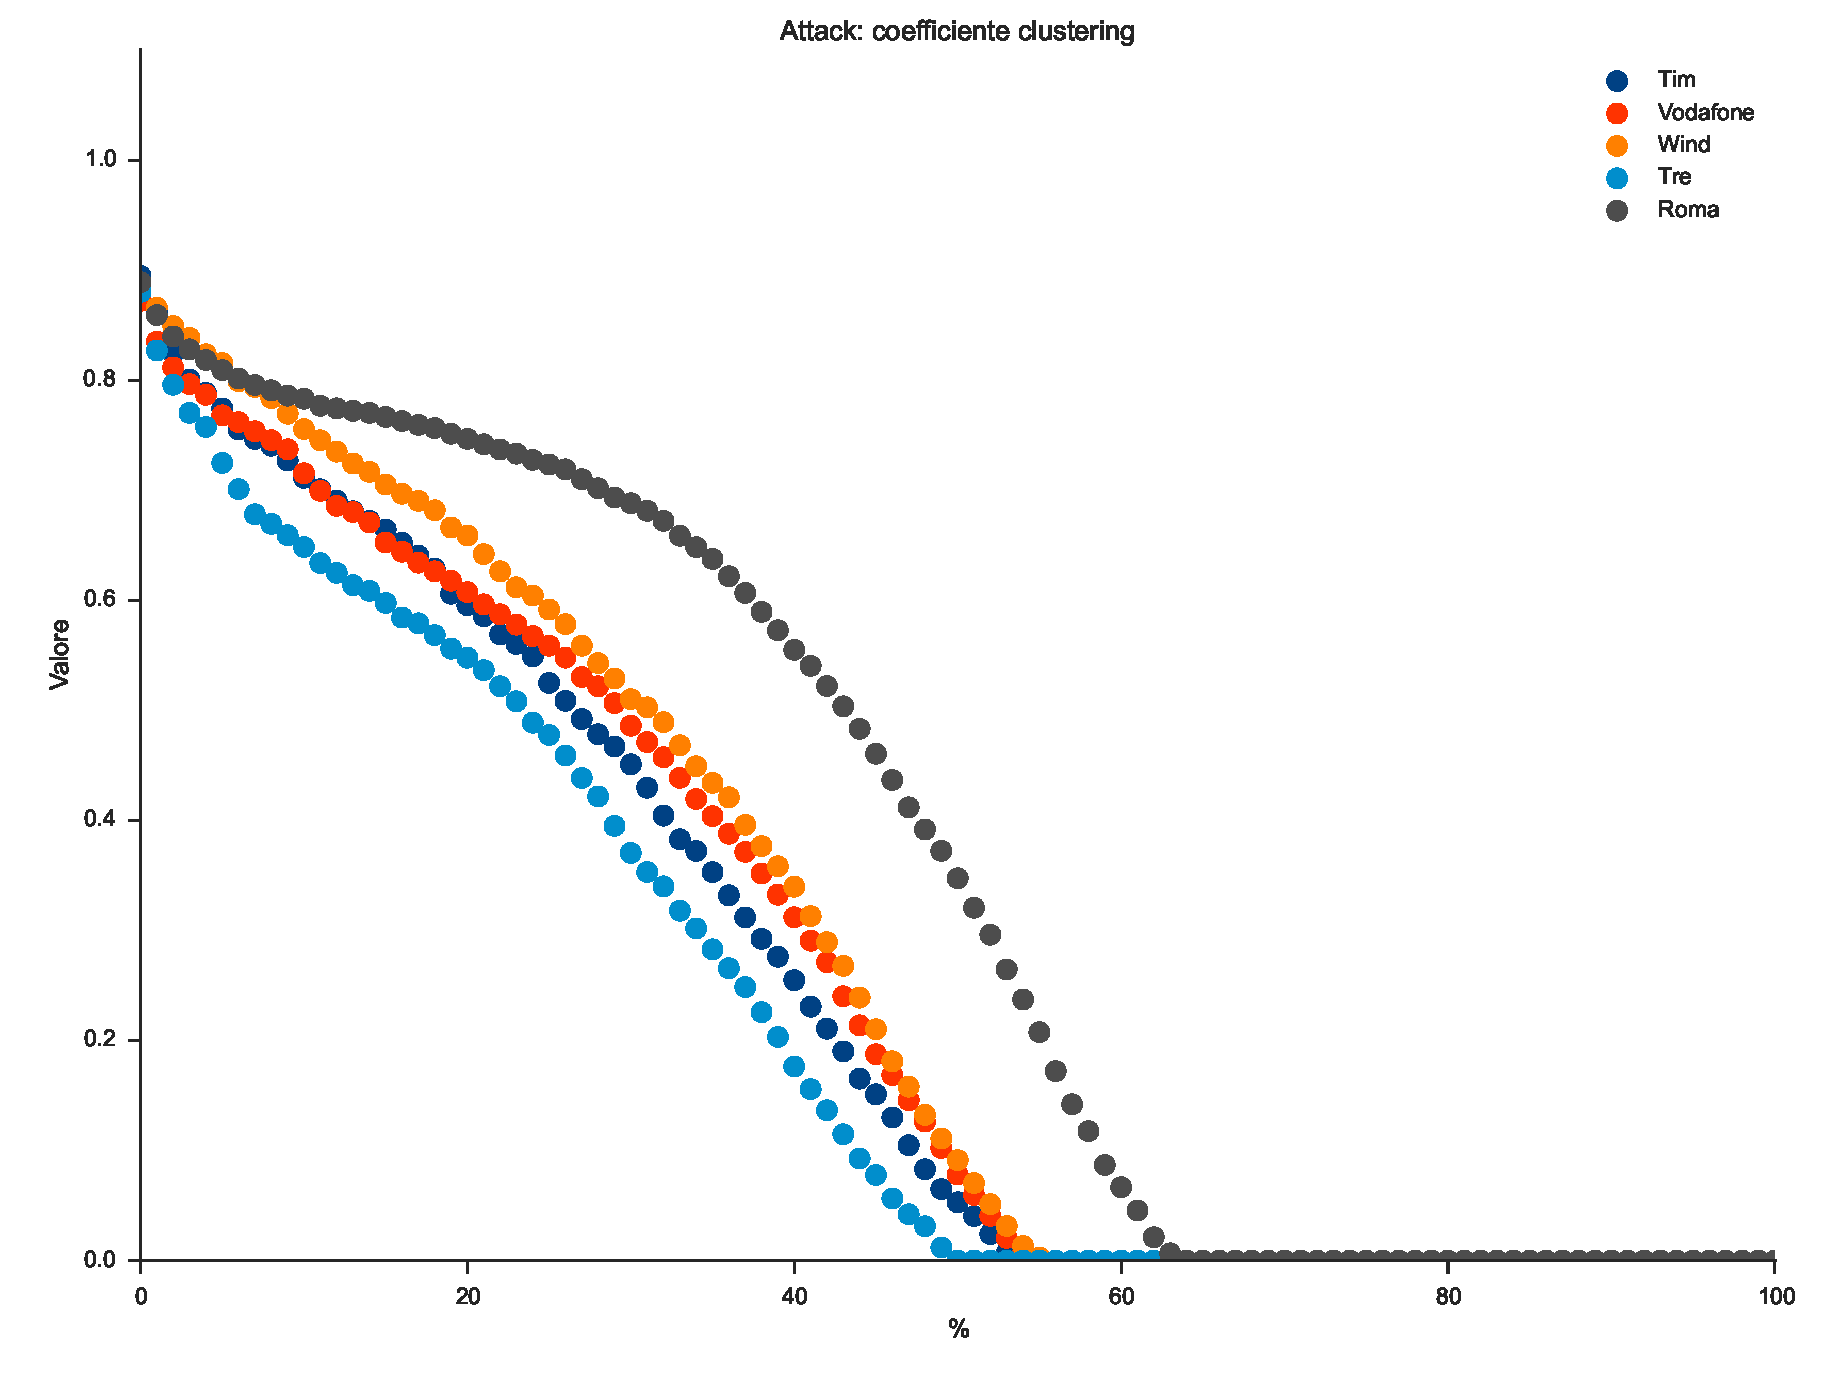
\includegraphics[width=0.46\textwidth]{./Immagini/Attack/gToolAttackC_Final}}
	\\
	\subfloat[$\langle l \rangle$]
	{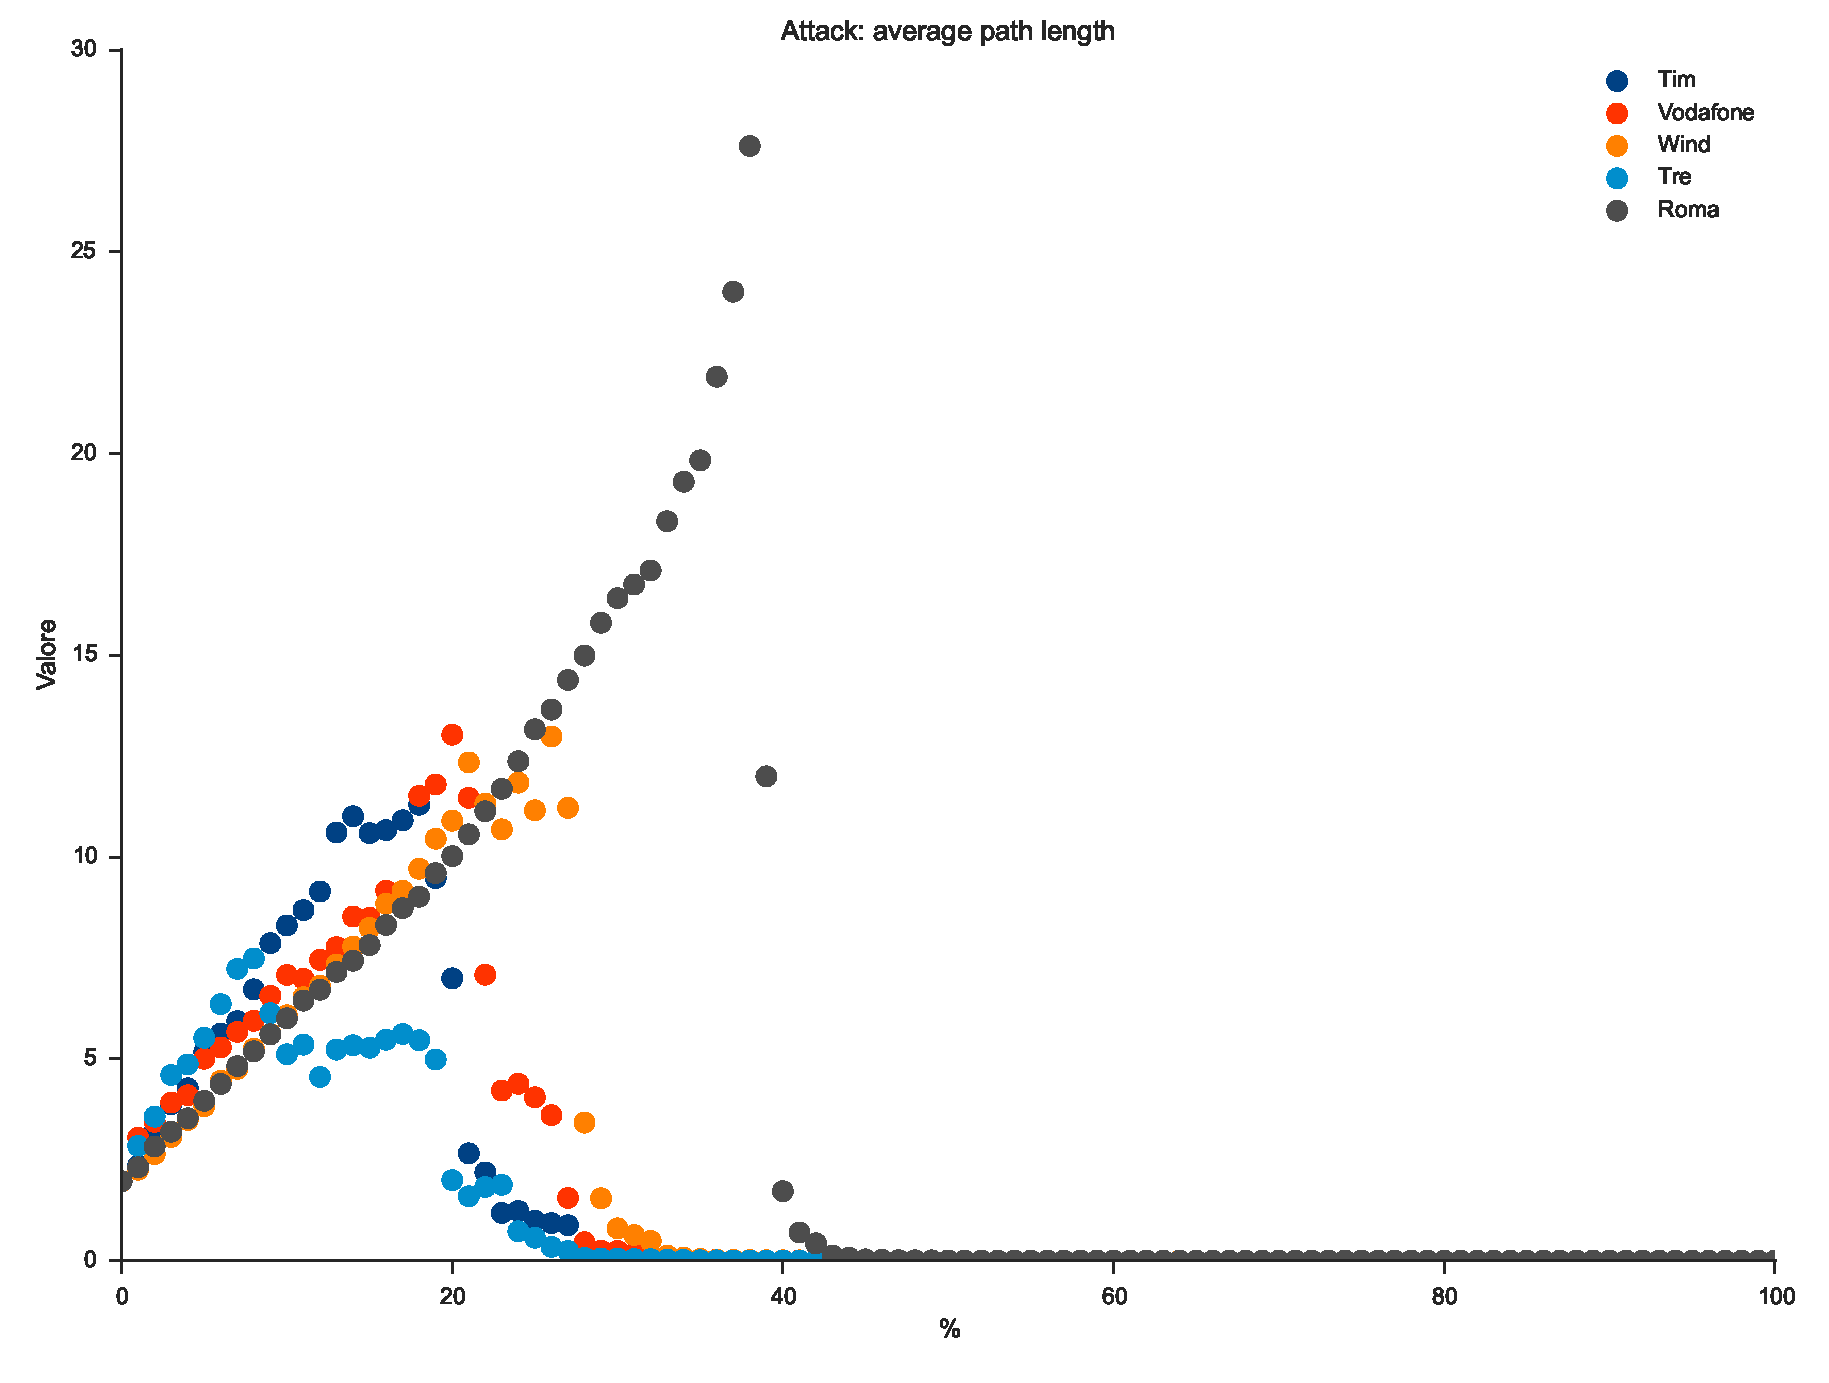
\includegraphics[width=0.46\textwidth]{./Immagini/Attack/gToolAttackl_Final}}
	$\;$
	\subfloat[$D$]
	{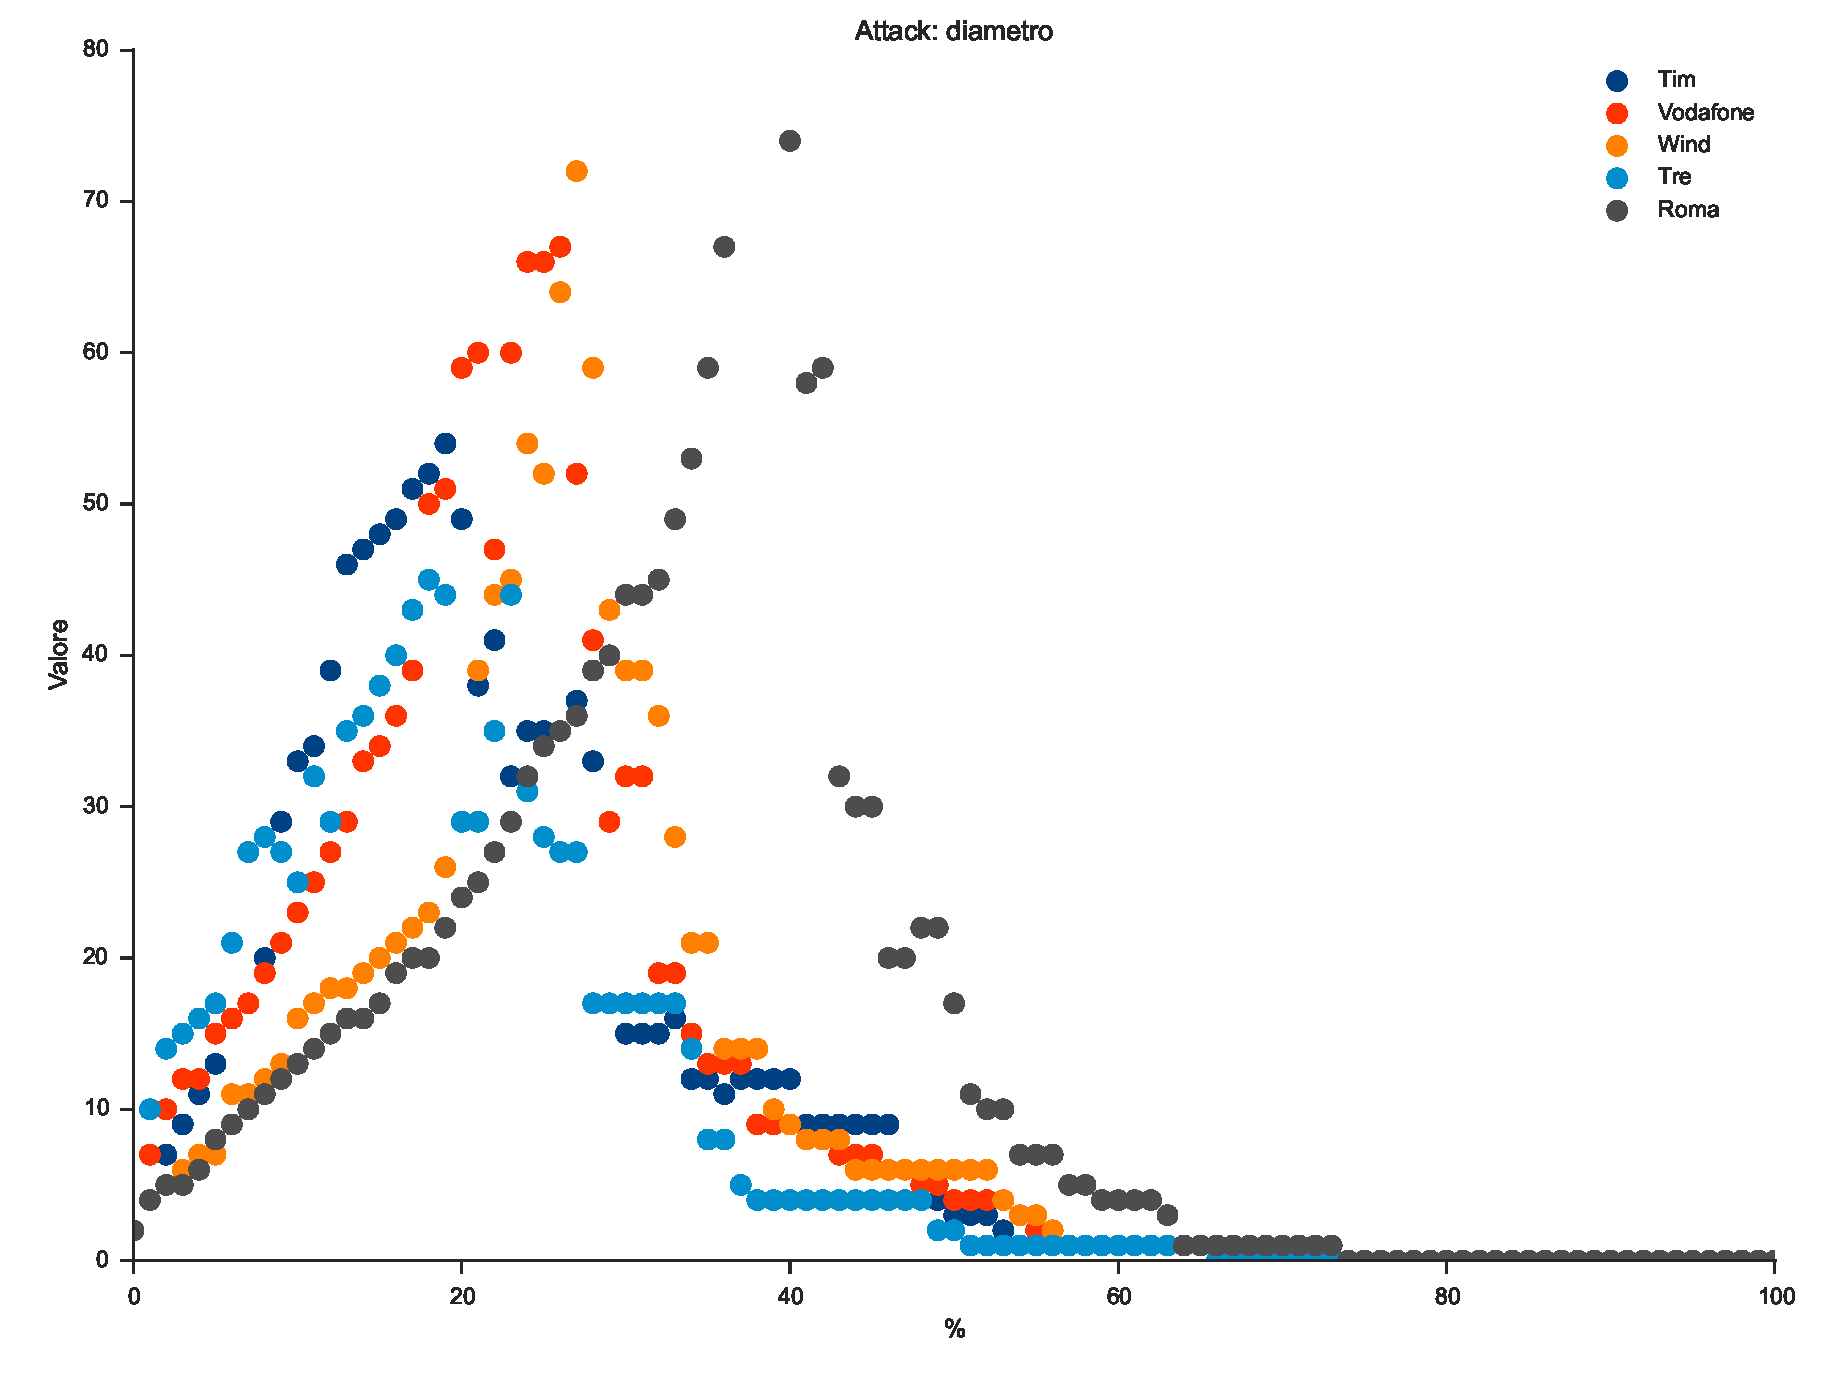
\includegraphics[width=0.46\textwidth]{./Immagini/Attack/gToolAttackD_Final}}
	\\
	\subfloat[$\langle k \rangle$]
	{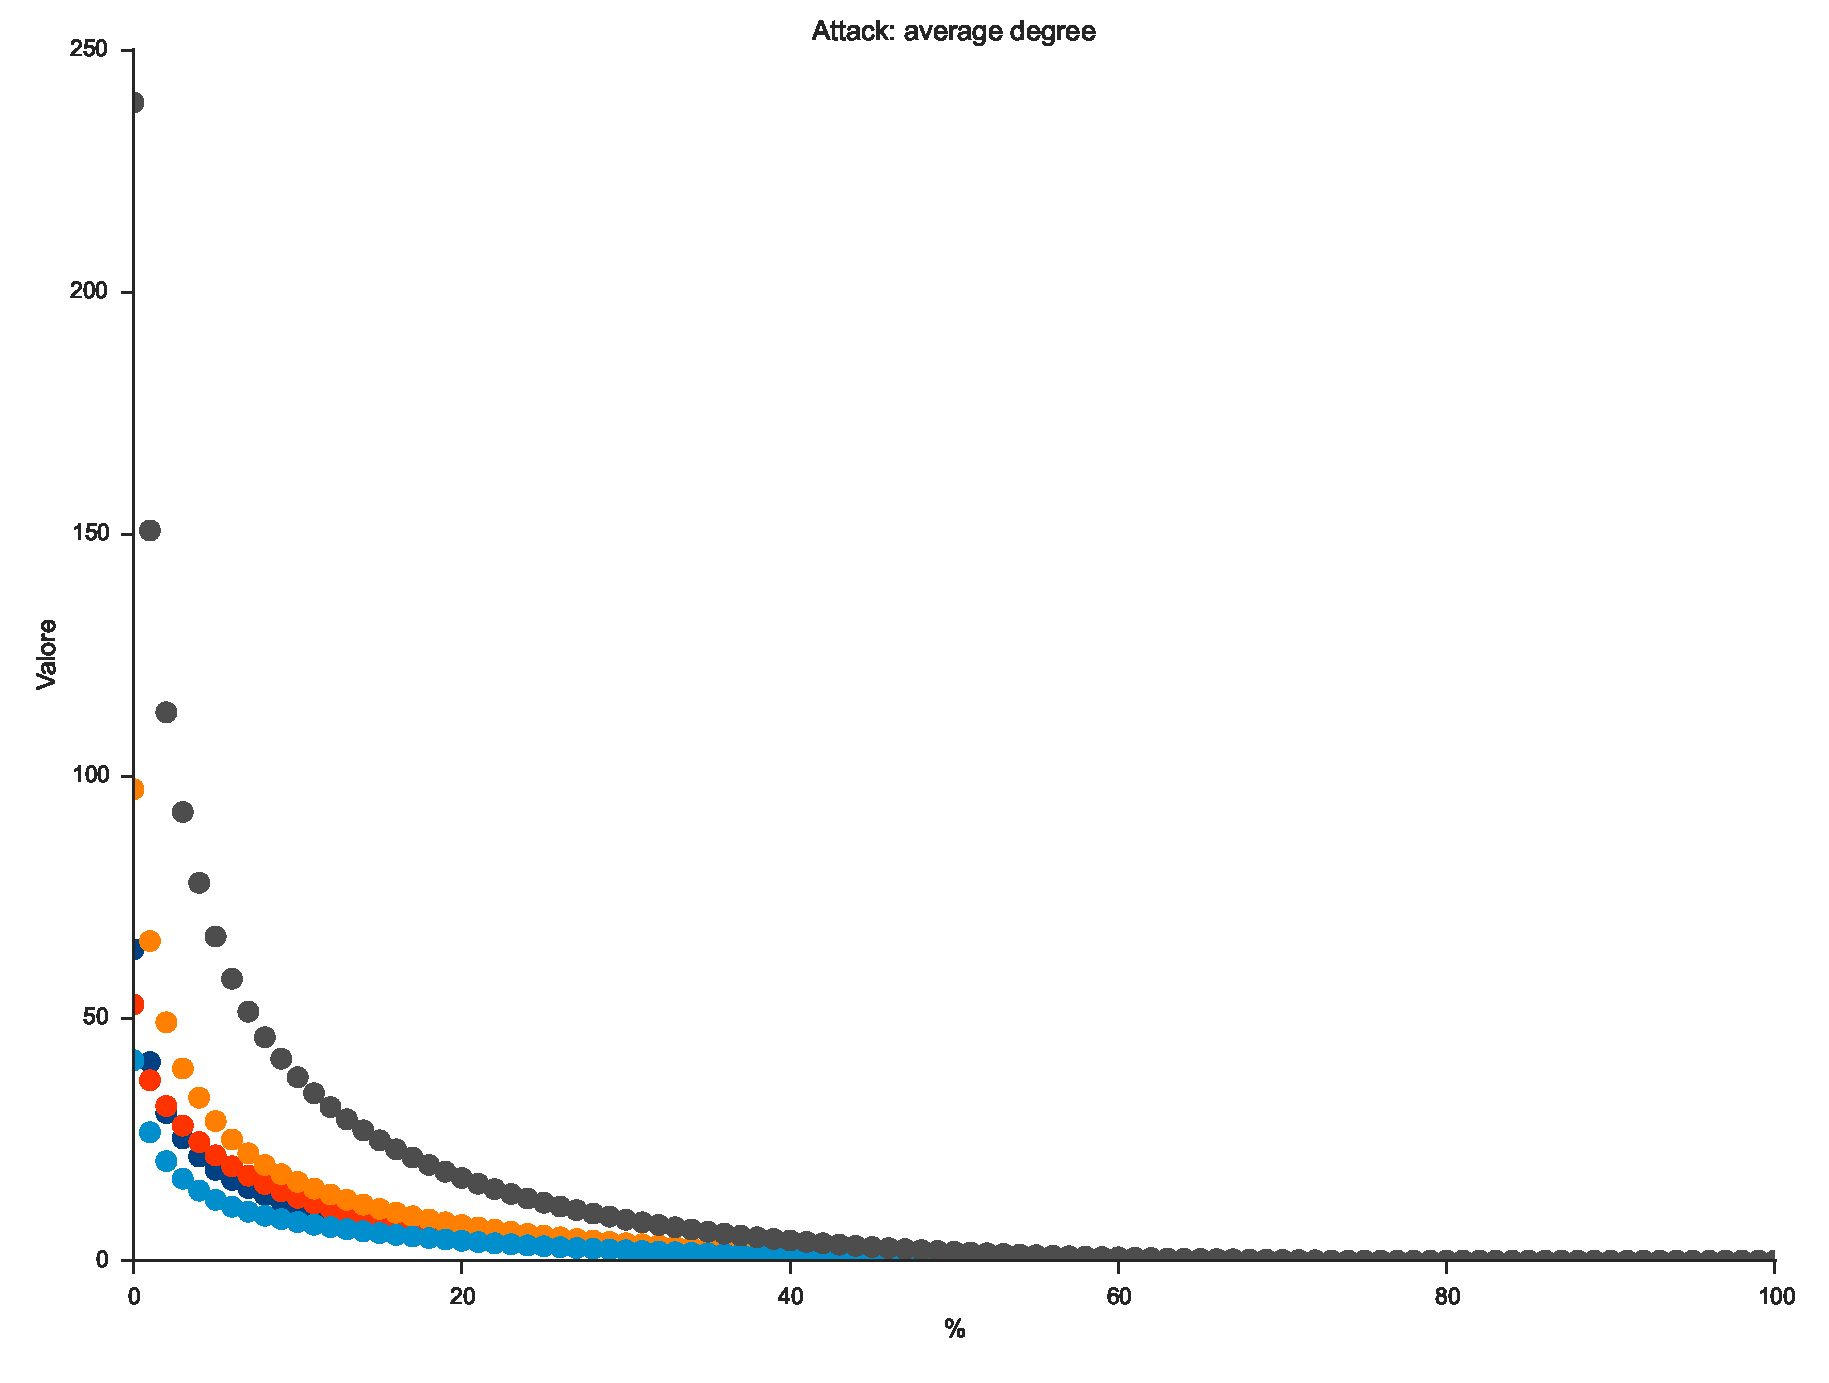
\includegraphics[width=0.46\textwidth]{./Immagini/Attack/gToolAttackk_Final}}
	$\;$
	\subfloat[$\langle k^2 \rangle/\langle k \rangle$]
	{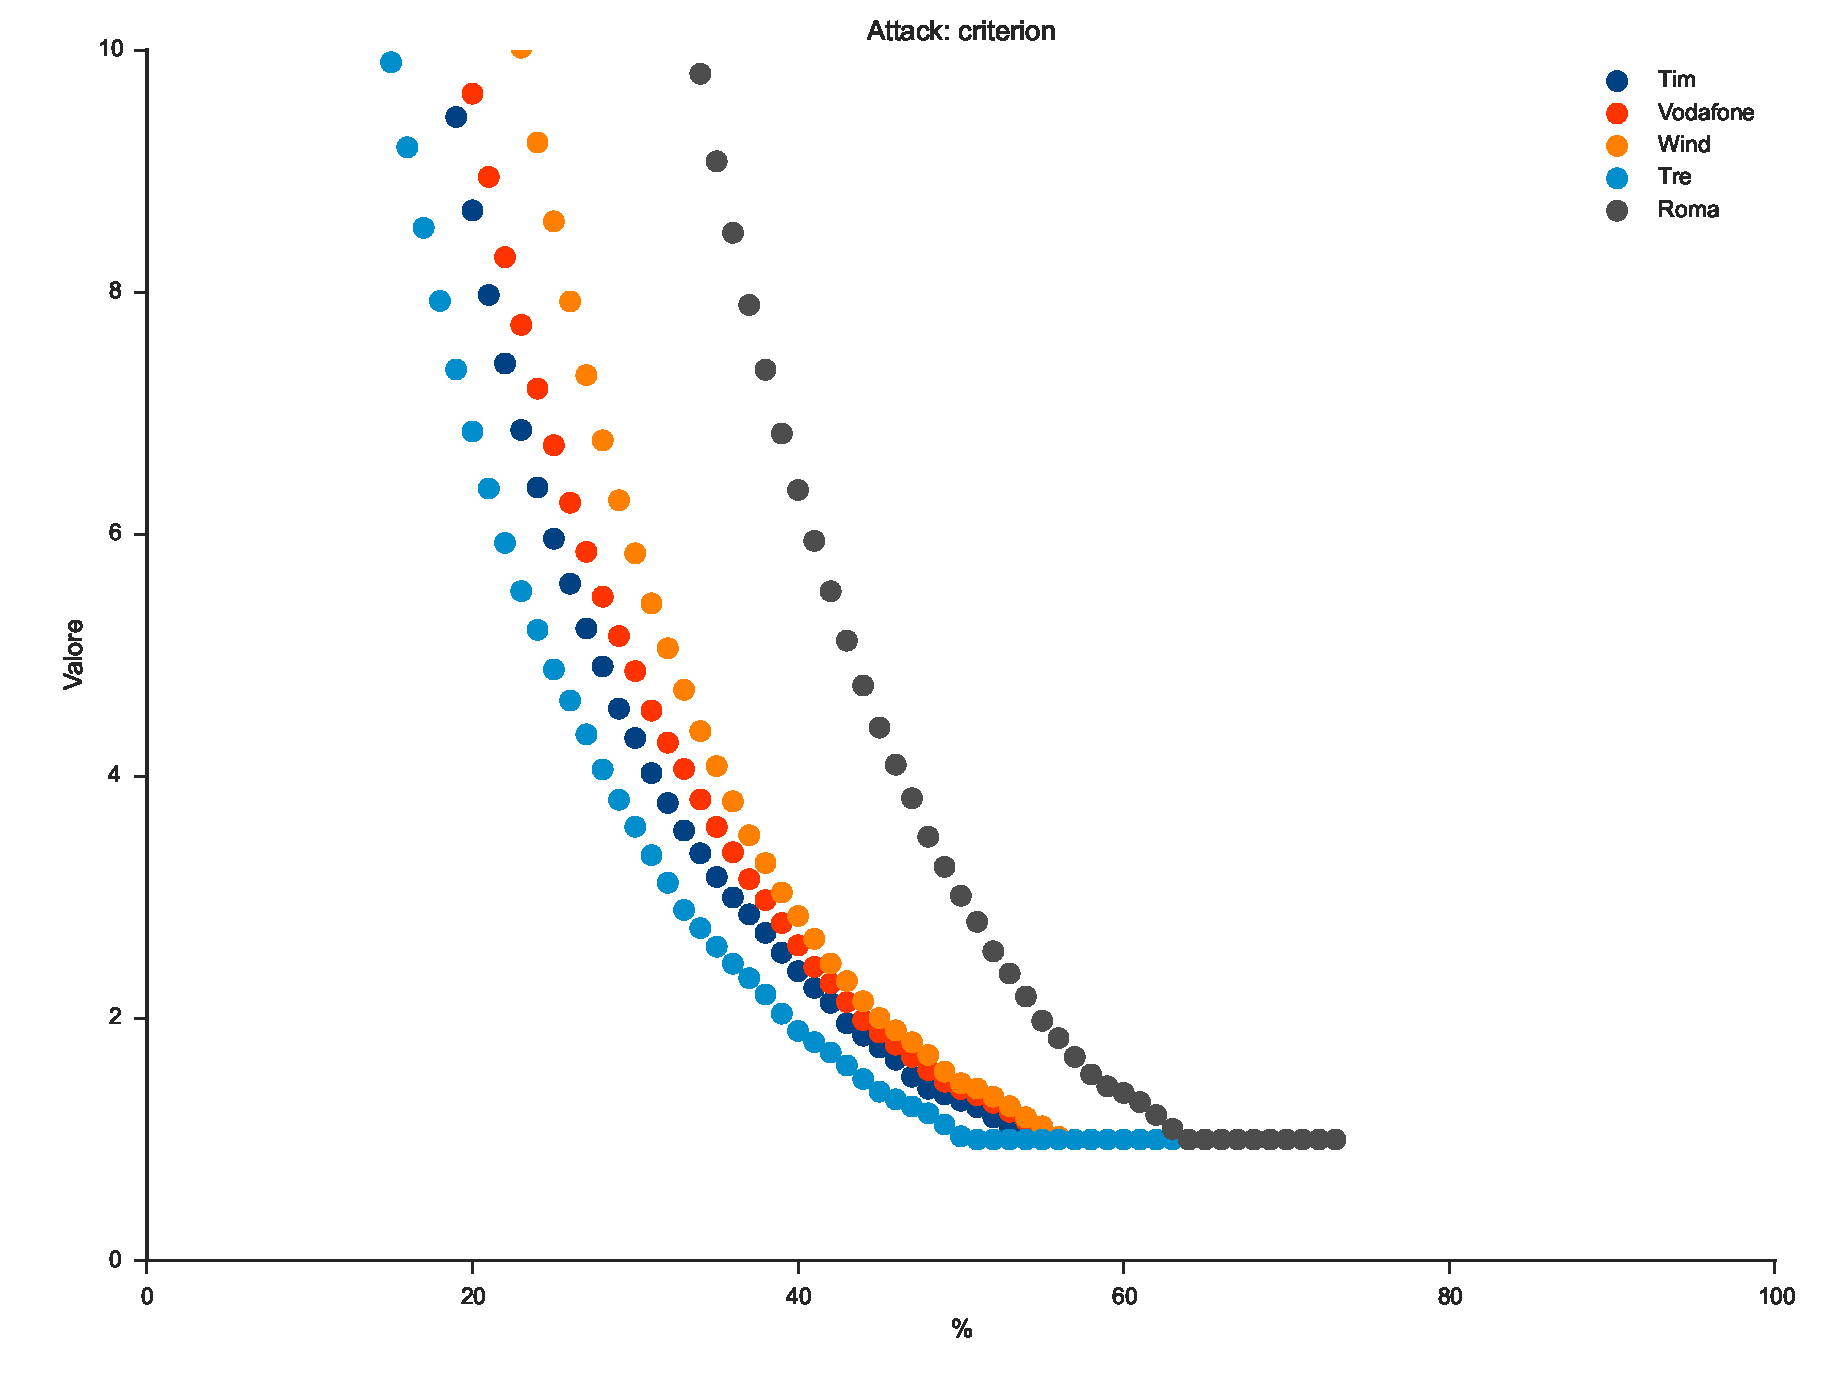
\includegraphics[width=0.46\textwidth]{./Immagini/Attack/gToolAttackc_Final}}
	\caption[Risultati attacco.]{Risultati per rimozione con massima efficienza}
	\label{fig:atak}
\end{figure}

\subsection{Conclusioni}
Come abbiamo visto, in regime di alta connettività, dal punto di vista percolativo si notano poco le differenze tra reti generate secondo un modello scale-free o random. La differenza si nota quando il grado medio della rete è più basso. Per esempio una rete random con $\langle k \rangle \sim 2$ ha $f\sim 50\%$, mentre una rete scale free con stesso $\langle k \rangle$ ha $f\sim 80\%$. Una spiegazione qualitativa sta nel fatto che con una distribuzione del grado a legge di potenza, i nodi meno connessi sono in larga maggioranza, quindi è meno probabile che un attacco random riesca a destrutturare la rete, rispetto a un grafo che abbia una $P(k)$ poissoniana. 

Un'altra cosa da notare è che a parità di $N$, una rete di Barabasi-Albert è molto più connessa di una di Erdos-Renyi. Nell'esempio sopra, infatti, con $N=100$ una la prima ha $\sim400$ link, mentre la seconda il doppio; per avere lo stesso numero di link la rete random ha bisogno di una $p \Rightarrow \langle k \rangle$ doppi. Questa differenza va attenuandosi con $N$ più grandi.

Uno studio percolativo su reti reali, quindi, non aiuta a identificare una eventuale invarianza di scala per reti molto grandi e connesse. Tuttavia può essere decisiva per reti più piccole, come piccole comunità, reti locali, proteine e alcuni ecosistemi: nonostante la bassa statistica, il comportamento di reti con pochi nodi possono essere distinti in maniera significativa da uno studio percolativo.

Nel caso di reti il cui funzionamento dipende dalla capacità dei nodi di gestire un certo carico, uno studio percolativo dovrebbe anche considerare l'eventualità che con la rimozione di alcuni nodi, altri vadano in sovraccarico e si scolleghino dalla rete (Motter \citeyear{Motter2002}, Zhao \citeyear{Zhao2004} e \citeyear{Zhao2005}, Wang \citeyear{Wang2009}). È il caso delle reti comunicative, come quelle telefoniche cellulari analizzate, o una ipotetica rete mesh costruita con i router wi-fi, ma anche ovviamente reti di distribuzioni elettriche, 
%valutare se lasciare o rimuovere
o alcuni ecosistemi dove una catena alimentare che veda la scomparsa di una specie causa una eccessiva riproduzione di una specie predata, che a sua volta porta altre specie all'estinzione.

Una possibile interessante applicazione dei metodi e degli strumenti usati per analizzare la rete di antenne di Roma potrebbe essere lo studio di città molto più grandi e densamente popolate (come New York o Tokyo), ma servirebbero capacità di calcolo e di memoria molto più grandi di quelle a nostra disposizione. Un altro possibile studio potrebbe essere verificare la possibilità di creare una rete distribuita e aperta con i router wi-fi. Avendo questi un raggio molto inferiore delle antenne cellulari, la rete sarebbe molto simile a un reticolo, quindi benché uno studio percolativo possa essere interessante, non lo sarebbe dal punto di vista delle reti complesse. 
%valutare se lasciare o rimuovere
Una rete di questo tipo sarebbe comunque un nuovo concetto di Internet, che potrebbe avere interessanti sviluppi su reti di altro tipo, per esempio sociali, correlate a essa.